\documentclass[11pt]{article}

% "review" for anonymous submission; "final" for camera-ready; "preprint" for a non-anonymous version.
\usepackage[review]{acl}

\usepackage{times}
\usepackage{latexsym}
\usepackage[T1]{fontenc}
\usepackage[utf8]{inputenc}
\usepackage{microtype}
\usepackage{inconsolata}
\usepackage{graphicx}
\usepackage{amsmath}
\usepackage{amssymb}
\usepackage{booktabs}
\usepackage{array}
\usepackage{fancyvrb}

\DeclareUnicodeCharacter{2212}{\ensuremath{-}}
\DeclareUnicodeCharacter{00D7}{\ensuremath{\times}}

\newcommand{\lit}[1]{\texttt{#1}}
\DefineVerbatimEnvironment{prompt}{Verbatim}{frame=single,fontsize=\footnotesize,xleftmargin=0.3em,xrightmargin=0.3em}

% Model count: single source of truth, updated when the replication models (Appendix A) finish.
\newcommand{\modelcountsentence}{A larger model from the same family, Qwen3-14B, replicated the
obsolete-state effect and the supersession contrast; its mention effect matched the superseded one (net
switch rates 0.169 and 0.167) rather than exceeding it. Gemma 3 4B did not meet the competence gate.}
\newcommand{\modelcount}{two models}
\newcommand{\modelcountconclusion}{Both confirmed models come from one family. Gemma 3 4B could not perform
the base task reliably enough to be evaluated, and other families remain untested.}

\title{Obsolete States Change Language-Model Decisions,\\and So Do Incidental Mentions}

\author{Anonymous ACL submission}

\begin{document}
\maketitle

\begin{abstract}
A model that reads an updated record can report the current value correctly and still let the old value
affect what it decides. We test whether that happens, and whether it happens \emph{because} the old value
was an assignment that has since been superseded. In synthetic access-control and routing records, the
current state, the decision policy and the correct action are held fixed while a single obsolete state is
edited so that it implies either the correct or the wrong action. Matched controls place the same word as
an assignment to an unrelated attribute that was later updated, as a word the same entity merely mentioned,
or as an unattached word. In a frozen confirmation on held-out wording (Qwen3-8B, 768 histories), the
obsolete state raised the wrong action's log-odds by 3.904 and 3.133 nats in the two tasks and flipped the
generated decision in about one history in six, almost always toward the wrong action (65 against 1 and 75
against 4 histories), including in routing conditions where the model retrieved both the current
(0.982--0.988) and the initial (0.990) state and decided correctly without history (0.953--0.961). The
effect is not specific to supersession: an incidental mention of the same word by the same entity moved
decisions as much in access and more in routing (net switches 0.294 against 0.185), and whether a
superseded assignment exceeded the mention control in score depended on the prompt template. A superseded
assignment exceeded an updated unrelated attribute in routing but not detectably in access. Finally,
the edit's effect on easy retrieval queries, a score-level sensitivity measure, added no information
about which decisions would fail beyond simple pre-decision predictors (log-loss gain $+0.0004$ nats,
95\% interval $[-0.0011, +0.0019]$). A second model, Gemma 3 4B, did not meet the task-competence gate,
so the results are for one model.
\end{abstract}

\section{Introduction}
\label{sec:intro}

Agents and assistants increasingly act on records that change: a user's clearance is revoked, a ticket is
rerouted, a preference is replaced. The record usually keeps the history, and the model is told that only
the latest entry counts. Retrieval benchmarks ask whether the model can then report the current value, and
recent work shows that old values do intrude on such reports, especially after many overwrites
\citep{wang2026unable,guo2026context,chattaraj2026dual}. A deployed system, however, rarely asks the model
to restate a value. It asks the model to \emph{use} it. Two questions follow that retrieval accuracy does
not answer. When a model can state the current value correctly, does the obsolete value still change the
decision it takes? And if it does, is the obsolete value acting as a superseded assignment of the queried
attribute, or simply as a word that occurs in the context near the entity?

The second question matters because the remedies differ. If the interference is tied to supersession, it
is a failure of state tracking, and update-aware memory, historical marking or attention routing toward the
current entry \citep{guo2026context} are the natural fixes. If any nearby mention of a decision-relevant
word does the same, the problem is contextual entrainment \citep{niu2025entrainment} reaching decisions.
Removing or marking stale entries would then leave much of it in place, and evaluations that only vary
update histories would misattribute it. The two accounts are not exclusive, and our design estimates
both.

\paragraph{Design.} We hold everything that should determine the decision fixed: the current state, the
policy that maps states to actions, the query, and the correct action. We edit one obsolete state. In one
member of each pair, the obsolete state implies the wrong action; in the other, it implies the correct
action. The difference in the model's preference for the wrong action between the two members is the
decision effect of the obsolete content, and the paired generated answers give its behavioral
counterpart (Figure~\ref{fig:example}). The same edit is repeated in matched constructions that keep the
word and its position but change its role: an assignment to a different attribute that was later updated,
a word the entity only mentioned, and a word attached to no entity. Before testing decisions, we check on
the same records that the model reports the current and the initial state correctly when asked.

\paragraph{Findings.} The experiment ran under a protocol frozen before the confirmation data were
generated, on a held-out prompt template, with Qwen3-8B. A larger model from the same family,
Qwen3-14B, was run on identical rows under a dated amendment, and Gemma 3 4B was attempted. The routing
task meets every competence criterion on the confirmation data in both Qwen models; the access task does not, and its estimates
are reported second and labeled. Three conclusions hold for both confirmed models, with one
model-specific difference:
\begin{enumerate}
  \item \textbf{Obsolete states change current decisions in models that track them correctly.} In the
  routing histories where the model retrieved the current and initial states and decided correctly without
  history, making the obsolete state imply the wrong action gave a net switch rate toward the wrong action
  of 0.158 (Qwen3-8B) and 0.165 (Qwen3-14B), almost never in reverse (\S\ref{sec:results-h1},
  \S\ref{sec:results-replication}).
  \item \textbf{Supersession adds decision pressure, and an incidental mention adds pressure of the same
  order.} In routing, a superseded assignment moved preference more than an updated assignment of an
  unrelated attribute, by 1.224 and 0.866 nats. The same word mentioned in passing by the same entity moved
  decisions as much as the superseded assignment in Qwen3-14B, and more in Qwen3-8B. Whether a mention
  \emph{exceeds} a superseded assignment therefore depends on the model, and in Qwen3-8B also on wording
  (\S\ref{sec:results-h2}).
  \item \textbf{A score-level sensitivity measure does not identify vulnerable items.} The edit's effect on
  easy retrieval queries was large, but in both models it added nothing beyond the pre-decision features
  under the specified logistic model (\S\ref{sec:results-h3}).
\end{enumerate}

\paragraph{What is and is not new.} That stale context interferes with answers is established
\citep{wang2026unable,guo2026context,qian2026forget,chao2026stale}, as is the fact that mentioned tokens
gain probability \citep{niu2025entrainment}. Our contribution is a controlled test that connects the two at
the level of decisions. We measure interference on policy decisions in open models, on items whose
current and historical states the model retrieves correctly. We use minimal-pair edits that hold the
correct action fixed, report both scores and generated answers, and include the matched controls needed
to ask whether supersession is the operative factor. We also report the negative result for a
sensitivity-based predictor and, in Appendix~\ref{app:history}, two measurement problems we found along
the way: chat-format events that the model never generates, and log-probabilities that change when tokens
are appended under 8-bit and bfloat16 inference.

\begin{figure*}[t]
\centering
\begin{prompt}
Read the dated record. Only the final assignment governs the decision.
Initially, EvbUnit0096A had routing state pending.        <- edited: pending | suspended
Initially, EvbUnit0096B had routing state suspended.
Later, EvbUnit0096A had archive tag restricted.
Finally, EvbUnit0096A had routing state restricted.
Later, EvbUnit0096B had archive tag restricted.
Finally, EvbUnit0096B had routing state pending.
Policy: state to bin: restricted -> B0, suspended -> B1, pending -> B2,
  active -> B3; bin to action: B0 -> EAST, B1 -> EAST, B2 -> WEST, B3 -> WEST
Apply the supplied rule to the final assignment of EvbUnit0096A; give its action.
Respond with exactly one label (EAST, WEST), with no other text.
\end{prompt}
\vspace{-0.5em}
{\small
\begin{tabular}{@{}ll@{}}
\toprule
Construction & Edited line (same word, same position) \\
\midrule
Superseded assignment & \lit{Initially, EvbUnit0096A had routing state pending.} \\
Other attribute, updated & \lit{Initially, EvbUnit0096A had archive tag pending.} \\
Mentioned by entity & \lit{Initially, EvbUnit0096A mentioned the word pending.} \\
Unattached word & \lit{Initially, the unassigned word was pending.} \\
\bottomrule
\end{tabular}}
\caption{One confirmation item (routing task, sequential order, held-out template; the annotation arrow is
not part of the prompt). The current state \lit{restricted} maps to \lit{EAST}. The obsolete state is
edited between \lit{pending} (implies \lit{WEST}, wrong) and \lit{suspended} (implies \lit{EAST}, correct);
everything else is identical. The table shows how the edited line reads in each construction. The decision
effect $D_c$ compares the model's preference for the wrong action across the two edits.}
\label{fig:example}
\end{figure*}

\section{Related work}
\label{sec:related}

\paragraph{Interference from updated values.} Proactive interference grows with the number of overwrites of
a key, and errors are mostly earlier values of the same key \citep{wang2025unable}. Models also retrieve
the first value of a key more reliably than the latest \citep{chattaraj2026dual,qiao2026retrieval}.
\citet{guo2026context} name the failure \emph{stale binding}. They find that almost all errors on current
value queries return an old value of the queried variable, that the current value stays linearly
recoverable on failures, that moving a historical mention near the query increases errors and historical
wording reduces them, and that test-time attention routing repairs most errors in 3--9B models. Their
decision scenarios, run with four closed reasoning models, showed no difference between full histories
and resolved snapshots. \citet{qian2026forget} and \citet{chao2026stale} evaluate forgetting and stale
memories in dialogue and agent settings. STALE in particular separates recognizing an update from applying
it in a later policy. Both are accuracy benchmarks with naturalistic text. Our setting differs in three
ways: a single update instead of long overwrite chains, decisions whose correct action is fixed by an
explicit policy, and matched minimal pairs with lexical controls. The failures we study sit below the
interference loads at which retrieval breaks.

\paragraph{Entrainment and distraction.} Tokens that appear in the context gain probability whether or
not they are relevant, random tokens included \citep{niu2025entrainment}. Irrelevant context also degrades
reasoning \citep{shi2023distracted}. Our entity-mention and unattached-word constructions measure this
effect in the update setting. The question we ask is whether a superseded assignment adds decision
pressure beyond it. \citet{yang2026compared} argue that counterfactual prompt edits are compound
treatments and must be compared against matched alternative edits rather than against no edit. Our design
follows that logic: each construction applies the same lexical edit, and the contrasts compare constructions.

\paragraph{Binding and state tracking.} Mechanistic work identifies how models bind attributes to entities
\citep{feng2024bind,gurarieh2026mixing,prakash2026lookbacks}. It also shows that models aggregate state
changes at query time rather than updating incrementally \citep{tang2026entities,kim2023entity}. These
accounts offer plausible reasons why lexical identity and position could matter more than assignment
history, but our experiments are behavioral and do not test them.

\paragraph{Knowledge conflicts.} Our records contain an intra-context conflict with an explicit temporal
resolution \citep{xu2024conflicts}. Related benchmarks ask for the value valid at a given time
\citep{yang2026conflicts}. That is our historical retrieval check, not our decision task.

\section{Task, constructions and estimands}
\label{sec:design}

\paragraph{Records and decisions.} Each history describes two entities. Each entity has an initial entry,
an update of a separate \emph{archive tag}, and a final assignment of the decision-relevant attribute
(Figure~\ref{fig:example}). A policy maps four states to two actions, two states per action. In the
\emph{access} task, clearance maps directly to \lit{APPROVE} or \lit{DENY}. In the \emph{routing} task,
the routing state maps to a bin and the bin to \lit{EAST} or \lit{WEST}. The model is asked for the action
implied by one entity's final assignment and must answer with exactly one label. Two vocabularies are used:
natural states (\lit{active}, \lit{pending}, \lit{restricted}, \lit{suspended}) and opaque states
(\lit{S1}--\lit{S4}). Natural labels carry prior meanings that the policy may contradict. Three orders
define the cells: \emph{sequential} (both initial entries, then both final blocks), \emph{interleaved}
(initial and final blocks alternate across entities), and \emph{competing} (interleaved, plus two
archived discussions that quote decision-relevant state words for the two entities). The factorial
crosses task, cell, vocabulary, correct action, historical order, current order and entity orientation:
192 histories per replicate. State-to-label assignments rotate so that every state appears in every role.
In every history the other entity's current state implies the wrong action. Confusing the two entities is
therefore always an error, but it is identical in both members of a pair and cancels in the paired
contrasts below.

\paragraph{Constructions.} For the queried entity, the obsolete line takes one of four forms, all with the
same edited word in the same slot:
\emph{superseded} (the queried attribute was initially assigned the word and later reassigned);
\emph{updated other attribute} (the archive tag was initially the word and was later updated);
\emph{entity mention} (the entity mentioned the word, with no assignment); and
\emph{unattached} (\lit{the unassigned word was}~\ldots). Every history also contains a
\emph{current-only} item with no initial lines, which measures whether the model can apply the policy at
all, and a \emph{live} item that edits the final assignment itself, which shows the size of a legitimate
change. The constructions share the policy, query, archive-tag update, final assignments and surrounding
text. They differ in syntax around the edited word, so the contrasts compare constructions as wholes,
not isolated semantic features.

\paragraph{Decision effect.} For a prompt $x$, let
$L(x) = \log P(a_{\mathrm{wrong}} \mid x) - \log P(a_{\mathrm{correct}} \mid x)$, where each action event
is the label exactly as the model writes it at the start of its turn, followed by the end-of-turn token.
For construction $c$ and history $h$, the two members differ only in the obsolete word: in member
$x^{-}_{h,c}$ it implies the wrong action, and in $x^{+}_{h,c}$ the correct one. The decision effect is
\begin{equation}
D_c = \frac{1}{|H|}\sum_{h \in H} \bigl[L(x^{-}_{h,c}) - L(x^{+}_{h,c})\bigr].
\end{equation}
$D_c > 0$ means the obsolete content pushes preference toward the action it implies. It is a preference
shift in nats, not an error rate. The two hypothesis contrasts are
$\Delta_{\mathrm{semantic}} = D_{\mathrm{superseded}} - D_{\mathrm{updated\,other}}$, which asks whether
the assignment's attribute matters, and
$\Delta_{\mathrm{mention}} = D_{\mathrm{superseded}} - D_{\mathrm{entity\,mention}}$, which asks whether
assignment adds anything to an incidental mention.

\paragraph{Generated switches.} With greedy decoding, a history scores $+1$ for construction $c$ if the
model answers wrongly under $x^{-}$ and not under $x^{+}$, $-1$ for the reverse, and $0$ otherwise. The
mean over histories is the \emph{net switch rate}, a value in $[-1, 1]$. The counts of histories with
$+1$ and $-1$ are reported as \emph{histories switched} to the wrong and to the correct action.

\paragraph{Retrieval checks.} On each record we also ask \emph{easy} queries for the current state of the
queried entity and of the other entity. For superseded items we ask for the \emph{initial} state, under an
introduction that announces both initial and final assignments. The answers are generated and parsed
strictly.

\paragraph{Easy-query sensitivity.} Let $w^{-}$ and $w^{+}$ be the two values of the edited word, and
let $m_{x}(w)$ be the log probability that easy query $q$, asked on record $x$, assigns to the answer
$w$ (summed over its spaced, unspaced and capitalized surface forms, scored as answer prefixes). Define
$E(q) = [m_{x^{+}}(w^{+}) - m_{x^{+}}(w^{-})] - [m_{x^{-}}(w^{+}) - m_{x^{-}}(w^{-})]$. Then
$R_{\mathrm{easy}} = E(\text{queried entity}) - E(\text{other entity})$ is a per-history, query-specific
sensitivity of retrieval scores to the edit. Hypothesis H3 asks whether $R_{\mathrm{easy}}$ helps predict
downstream failures beyond features that are available before the decision query is asked.

\section{Protocol}
\label{sec:protocol}

\paragraph{Model and runtime.} Qwen3-8B \citep{yang2025qwen3} at a pinned revision
(Appendix~\ref{app:repro}), with thinking disabled through the chat template. Inference ran in float32
without quantization on one GPU. We chose float32 after finding that 8-bit and bfloat16 inference made
the log probability at a fixed position change by up to 0.843 and 0.875 nats when tokens were appended
after it. Float32 gave exactly zero (Appendix~\ref{app:precision}). Action events were scored with a
key--value-cache scorer. Before each run, the scorer was checked against one full forward pass per event
on identical prompts (maximum difference $5.08\times10^{-5}$ nats against a tolerance of 0.02). Answers
were generated greedily with at most 16 new tokens and parsed strictly: an answer counts only if, after
stripping outer whitespace, it is exactly one allowed label.

\paragraph{Splits and gate.} Three disjoint splits were generated from separate seeds and separate
entity-name pools. A development split (192 histories) was used only to check competence and answer
formats. A frozen gate split (384 histories) decided eligibility. The confirmation split (768 histories,
8{,}448 records, 11 per history) used a held-out paraphrase of the introduction and query. A task-cell
was \emph{competent} if strict direct retrieval of the current state was at least 0.95, current-only
decision accuracy at least 0.90, and invalid answers at most 0.05. Confirmation data were generated only
after the gate, recomputed from its saved scores, showed at least one competent cell. All cells are
reported. Task-level estimates average the fixed grid, and estimates from non-competent cells are labeled
as such.

\paragraph{Hypotheses and statistics.} The protocol fixed two primary hypotheses per task: H1,
$D_{\mathrm{superseded}} > 0$; and H2, $\Delta_{\mathrm{semantic}} \neq 0$, two-sided. Both use 97.5\%
percentile intervals from a history bootstrap (2{,}000 draws, fixed seed), Bonferroni-adjusted over the
two tasks. Secondary outcomes use unadjusted 95\% intervals: $\Delta_{\mathrm{mention}}$, the other
construction effects, net switch rates, and H3. Histories are the resampling unit. Both members, all
constructions and all queries of a history stay together. The two tasks are never pooled, and an
interval that includes zero is reported as inconclusive, not as evidence of no effect.

\paragraph{Prediction (H3).} Predictors that are available before the decision query is asked: the easy
query's margin between the current and the historical state, the historical candidate's log mass, easy
confidence, the edited token's position, prompt length, and design indicators. The comparison adds
$R_{\mathrm{easy}}$ to these. The outcome is a strict downstream failure on the historical constructions.
Models are L2-regularized logistic regressions ($C=1$, no tuning) evaluated by five-fold cross-validation
with folds grouped by history. Out-of-fold log loss with and without $R_{\mathrm{easy}}$ is compared by a
paired history bootstrap. The downstream answer's own confidence is reported separately as a
contemporaneous reference, not as a predictor, because it comes from the decision query itself.

\paragraph{Protocol history.} The confirmation protocol is the second redesign of a design that was
frozen before any model was run. The first version scored action events that the model never produces
and was corrected before inference. The second failed its competence gate because a trailing
\lit{Answer:} line made the model echo the prefix. The redesign changed only that line, the seeds and
the name pools. Appendix~\ref{app:history} lists every change and when it was made. The protocol records
are internal and dated. We call them \emph{frozen before confirmation}, not preregistered.

\section{Results}
\label{sec:results}

All numbers in this section come from the frozen confirmation (Qwen3-8B, held-out template, 384 histories
per task) unless marked otherwise.

\subsection{Competence}
\label{sec:results-competence}

\begin{table}[t]
\centering
\small
\setlength{\tabcolsep}{4pt}
\begin{tabular}{@{}lcccc@{}}
\toprule
Cell & Direct & No history & History & Competent \\
\midrule
routing seq.  & 0.988 & 0.953 & 0.858 & yes \\
routing int.  & 0.986 & 0.961 & 0.868 & yes \\
routing comp. & 0.982 & 0.953 & 0.846 & yes \\
\midrule
access seq.   & 0.916 & 0.867 & 0.831 & no \\
access int.   & 0.945 & 0.875 & 0.858 & no \\
access comp.  & 0.908 & 0.859 & 0.867 & no \\
\bottomrule
\end{tabular}
\caption{Strict accuracy on the confirmation data. \emph{Direct}: current state of the queried entity,
asked directly. \emph{No history}: decision on the current-only item. \emph{History}: decision over all
historical-construction items. Competent: direct $\ge 0.95$, no history $\ge 0.90$, invalid $\le 0.05$.
No answer was invalid.}
\label{tab:competence}
\end{table}

On the confirmation data, the routing cells meet all competence criteria and the access cells do not, mainly because current-only
decisions fall short of 0.90 (Table~\ref{tab:competence}). Asked for the \emph{initial} state on the
superseded items, the model answered correctly in 0.990 of routing and 0.973 of access cases. In routing,
then, the model reports the current state, reports the initial state, and applies the policy without
history at or above 0.95. Access results are reported below as fixed-grid averages over cells that do not
meet the competence criteria.

\subsection{Obsolete states change decisions}
\label{sec:results-h1}

\begin{figure*}[t]
\centering
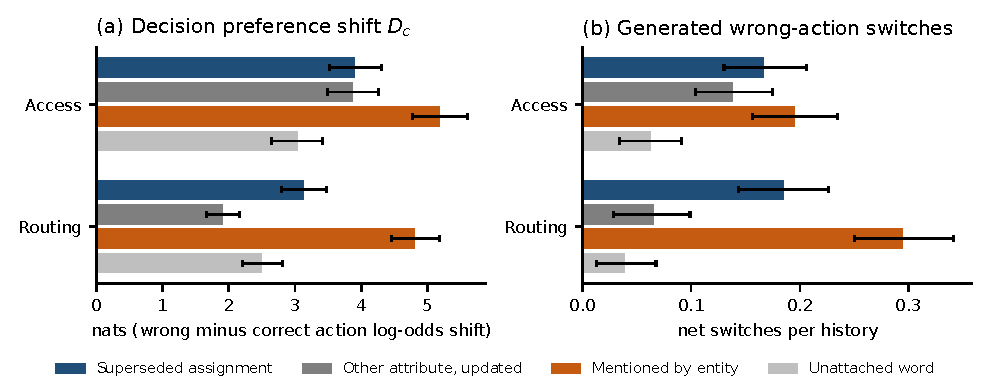
\includegraphics[width=\textwidth]{figures/constructions.pdf}
\caption{Decision effects by construction (confirmation, 384 histories per task, 95\% history-bootstrap
intervals). (a) $D_c$: increase in the wrong action's log-odds when the edited word implies the wrong
rather than the correct action. (b) Net switch rate toward the wrong action (mean over histories of $+1$,
$0$ or $-1$). Routing cells meet the competence criteria on the confirmation data; access cells do not.}
\label{fig:constructions}
\end{figure*}

H1 is supported in both tasks. In routing, when the superseded state implied the wrong action rather
than the correct one, the wrong action's log-odds rose by $D_{\mathrm{superseded}} = 3.133$ nats
(97.5\% interval $[2.743, 3.516]$). In access, where cells do not meet the competence criteria, the shift
was $3.904$ $[3.474, 4.346]$. For scale, editing the \emph{current} state itself, which legitimately
changes the correct action, moved the same quantity by $-8.197$ (routing) and $-10.100$ nats (access).

The shift reaches generated answers. In routing, the net switch rate toward the wrong action was $0.185$
$[0.143, 0.227]$: 75 histories switched to the wrong action and 4 to the correct one. In each routing
cell, it was between 0.164 and 0.227 (Table~\ref{tab:switch-cells}). In access it was $0.167$
$[0.130, 0.206]$ (65 against 1). Figure~\ref{fig:competence} shows the same effect as accuracy. In every
routing cell, decisions were correct in 0.906--0.953 of histories when the superseded state implied the
correct action, and in 0.727--0.750 when it implied the wrong one. The same records gave current- and
initial-state retrieval at or above 0.98.

\paragraph{Histories the model demonstrably tracks.} Aggregate retrieval accuracy does not show that the
switching histories are ones the model reads correctly. We therefore kept a history only if three
conditions held on the same records: the model retrieved the current state correctly under both members
of the pair, retrieved the initial state correctly under both superseded members, and decided the
current-only item correctly. This kept 348 of 384 routing histories for the superseded construction
(Table~\ref{tab:joint}). In them, the net switch rate toward the wrong action was $0.158$
$[0.118, 0.198]$: 58 histories switched to the wrong action and 3 to the correct one. The preference
shift was $2.990$ nats $[2.661, 3.342]$. Each routing cell keeps a net switch rate between 0.129 and
0.202. The effect is therefore not carried by histories in which the model misreads the record. In
access, the same restriction keeps 284 of 384 histories and gives a net switch rate of $0.176$
$[0.134, 0.218]$ (50 against 0).

\begin{table}[t]
\centering
\small
\setlength{\tabcolsep}{3pt}
\resizebox{\columnwidth}{!}{%
\begin{tabular}{@{}lcccc@{}}
\toprule
& Kept & $D_{\mathrm{superseded}}$ & Net switch rate & Switched \\
\midrule
routing seq.  & 118/128 & 2.959 & 0.144 $[0.076, 0.220]$ & 19 / 2 \\
routing int.  & 114/128 & 3.252 & 0.202 $[0.132, 0.281]$ & 24 / 1 \\
routing comp. & 116/128 & 2.764 & 0.129 $[0.069, 0.190]$ & 15 / 0 \\
routing, all  & 348/384 & 2.990 & 0.158 $[0.118, 0.198]$ & 58 / 3 \\
\midrule
access, all   & 284/384 & 4.059 & 0.176 $[0.134, 0.218]$ & 50 / 0 \\
\bottomrule
\end{tabular}}
\caption{Superseded construction, restricted to histories with correct current-state retrieval under both
members, correct initial-state retrieval under both members, and a correct current-only decision. Kept:
histories retained out of those in the cell. Switched: histories switched to the wrong / to the correct
action. 95\% history-bootstrap intervals. Retained sets differ slightly across constructions because
condition (i) is checked per construction. Condition (ii) is checked on the history's superseded members for
every construction, because the initial-state query is asked only there.}
\label{tab:joint}
\end{table}

\begin{figure*}[t]
\centering
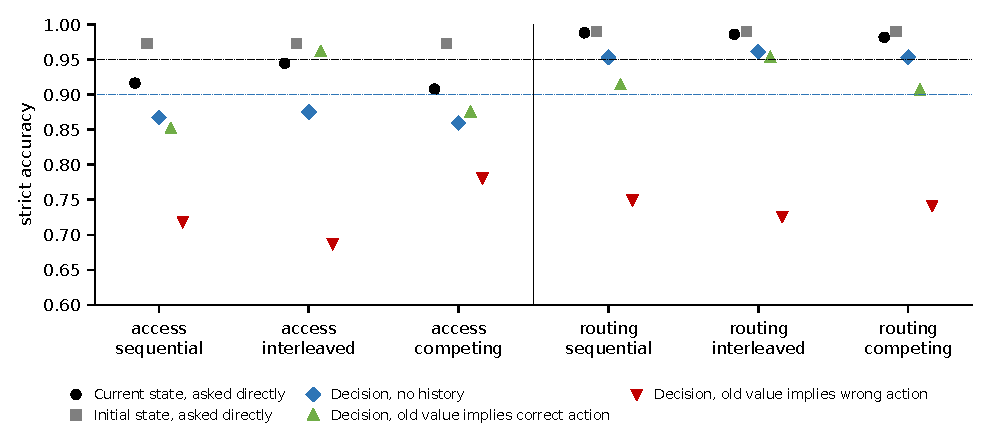
\includegraphics[width=\textwidth]{figures/competence.pdf}
\caption{Retrieval and decision accuracy on the same confirmation records, per cell. Initial-state
retrieval is reported per task. Routing (left) meets the competence criteria on the confirmation data; access (right) does not.}
\label{fig:competence}
\end{figure*}

\subsection{Supersession adds pressure; a mention adds comparable pressure}
\label{sec:results-h2}

This section reports Qwen3-8B, where a mention adds more pressure than a superseded assignment;
\S\ref{sec:results-replication} shows that in Qwen3-14B it adds comparable pressure. H2 compares the
superseded assignment with an assignment of the same word to a different attribute that was later updated. It is supported in routing, $\Delta_{\mathrm{semantic}} = +1.224$ $[0.973, 1.485]$, with
generated switches agreeing ($+0.120$ $[0.076, 0.164]$). In routing, then, the attribute that was
superseded matters. In access (non-competent cells) the contrast is inconclusive: $+0.035$
$[-0.318, 0.400]$, switches $+0.029$ $[-0.016, 0.073]$.

The mention control, a secondary outcome, shows that supersession is not the largest source of pressure
in Qwen3-8B.
When the same entity only \emph{mentioned} the word, the effect was larger than for the superseded
assignment. In routing, $D_{\mathrm{entity\,mention}} = 4.807$ against $3.133$, so
$\Delta_{\mathrm{mention}} = -1.675$ $[-1.896, -1.441]$. Net switches were $0.294$ (113 to wrong, 0 to
correct) against $0.185$, difference $-0.109$ $[-0.156, -0.065]$. In access, $5.182$ against $3.904$
($\Delta_{\mathrm{mention}} = -1.278$ $[-1.579, -0.977]$). Switches there were $0.195$ (76 against 1)
against $0.167$, an inconclusive difference. A word attached to no entity still shifted preference
substantially, by $2.496$ (routing) and $3.043$ nats (access), but rarely changed a generated decision
($0.039$ and $0.062$). Score shifts of similar size can thus have very different behavioral
consequences. The ordering holds in the restricted routing histories of Table~\ref{tab:joint}. Net switch
rates there are $0.278$ for the mention, $0.158$ for the superseded assignment, $0.048$ for the updated
unrelated attribute and $0.034$ for the unattached word.

Across four earlier, non-confirmatory splits, $\Delta_{\mathrm{mention}}$ never favored the superseded
assignment, but its size varied with the template (Appendix~\ref{app:tables}, Figure~\ref{fig:replication}).

\subsection{Easy-query sensitivity adds nothing to failure prediction}
\label{sec:results-h3}



The edit strongly affected easy retrieval scores: the mean $R_{\mathrm{easy}}$ on superseded items was
$8.096$ nats in access and $10.878$ in routing. That sensitivity added nothing beyond the pre-decision
features under the specified logistic model (Table~\ref{tab:h3} in Appendix~\ref{app:tables}). Pre-decision features reduced log loss from $0.414$ to
$0.346$ and reached AUROC $0.780$. Adding $R_{\mathrm{easy}}$ changed log loss by $+0.0004$ nats,
interval $[-0.0011, 0.0019]$; the upper end is under 3\% of what the simple features already gain. The
result is the same in each task and for the wrong-answer outcome. It replicates in Qwen3-14B: AUROC
$0.684$ without and $0.685$ with $R_{\mathrm{easy}}$, log-loss gain $-0.0001$ $[-0.0027, 0.0022]$. Within
this design,
$R_{\mathrm{easy}}$ describes how retrieval scores respond to the edit; it does not diagnose decision
vulnerability.

\subsection{Replication in Qwen3-14B, and a model that was not eligible}
\label{sec:results-replication}
\label{sec:results-gemma}

\begin{table*}[t]
\centering
\small
\setlength{\tabcolsep}{4pt}
\resizebox{\textwidth}{!}{%
\begin{tabular}{@{}llccccc@{}}
\toprule
Model & Task (competent cells) & $n$ & $D_{\mathrm{superseded}}$ & $\Delta_{\mathrm{semantic}}$ & $\Delta_{\mathrm{mention}}$ & Net switch rate \\
\midrule
Qwen3-8B & routing (comp., int., seq.) & 384 & $+3.133$ {\scriptsize $[+2.743, +3.516]$} & $+1.224$ {\scriptsize $[+0.973, +1.485]$} & $-1.675$ {\scriptsize $[-1.896, -1.441]$} & $+0.185$ {\scriptsize $[+0.143, +0.227]$} \\
Qwen3-8B & access & \multicolumn{5}{l}{no competent cell} \\
\midrule
Qwen3-14B & routing (comp., int., seq.) & 384 & $+4.785$ {\scriptsize $[+4.244, +5.354]$} & $+0.866$ {\scriptsize $[+0.417, +1.328]$} & $+0.248$ {\scriptsize $[-0.117, +0.601]$} & $+0.167$ {\scriptsize $[+0.130, +0.206]$} \\
Qwen3-14B & access & \multicolumn{5}{l}{no competent cell} \\
\midrule
Gemma 3 4B & \multicolumn{6}{l}{not eligible: no competent cell at the gate} \\
\bottomrule
\end{tabular}}
\caption{Confirmation results per model, on the task-cells that met the competence criteria \emph{on the confirmation data} (the rule used in the text and in Table~\ref{tab:competence}). $D$ and $\Delta$ in nats; $D_{\mathrm{superseded}}$ and $\Delta_{\mathrm{semantic}}$ with 97.5\% intervals, $\Delta_{\mathrm{mention}}$ and the superseded net switch rate with 95\% intervals (history bootstrap). Models are reported separately, never pooled. The replication amendment defined competent cells by each model\textquoteright s frozen gate (Table~\ref{tab:models-gate}); gate-rule estimates are in Appendix~\ref{app:tables}.}
\label{tab:cross-model}
\end{table*}


Qwen3-14B was added under an amendment dated before any of its data were scored, with the same rows, rules
and runtime (Appendix~\ref{app:history}). Its frozen gate passed in all three routing cells and in no access
cell (Table~\ref{tab:models-gate}). On the confirmation, routing retrieval was 0.989--0.997 for the current
state and 0.997 for the initial state. Current-only decisions were 0.977--0.992 correct.

Table~\ref{tab:cross-model} compares the two models on the cells competent on the confirmation data. The obsolete-state effect
replicates. In routing, $D_{\mathrm{superseded}} = 4.785$ nats and the net switch rate is $0.167$ (67
histories switched to wrong, 3 to correct). In the routing histories Qwen3-14B demonstrably tracks (376 of
384), it is $0.165$ $[0.128, 0.205]$ (Table~\ref{tab:joint-by-model}). Supersession again adds preference
over an updated unrelated attribute: $\Delta_{\mathrm{semantic}} = +0.866$ $[0.417, 1.328]$ in routing.
In generated switches, however, the two constructions are close in this model ($0.167$ against $0.146$).
The mention result differs from Qwen3-8B. In Qwen3-14B the mention moves routing decisions as much as the
superseded assignment does: net switch rates are $0.169$ against $0.167$ over all routing histories, and
$0.168$ against $0.165$ in the tracked histories (Table~\ref{tab:joint-by-model}), with
$\Delta_{\mathrm{mention}} = +0.248$ $[-0.117, 0.601]$, an inconclusive difference. In access
(non-competent cells) the superseded assignment moved preference more than the mention
($\Delta_{\mathrm{mention}} = +0.845$ $[0.425, 1.255]$). In both models, then, an incidental mention
produces interference of the same order as a superseded assignment. Whether it exceeds it is
model-specific.

Gemma 3 4B was added under a model list frozen before any of its data were scored. On the gate split, no
cell met the criteria: current-only decision accuracy was 0.609--0.719, direct retrieval 0.916--0.964
(Table~\ref{tab:models-gate}), while initial-state retrieval in development was 0.984. Gemma reads these
records but does not apply the policy reliably, so no confirmation split was generated for it. This is an
eligibility result, not evidence for or against stale-state interference in Gemma.

\section{Discussion}
\label{sec:discussion}

\paragraph{What the evidence supports.} In two models that report both the current and the initial state
correctly, an obsolete state still moves routing decisions toward the action it implies. The net switch
rate is 0.158 (Qwen3-8B) and 0.165 (Qwen3-14B) in the histories where the model retrieved both states and
decided correctly without history. Stale-value interference, documented for value queries
\citep{guo2026context,wang2026unable}, thus also reaches single-step policy decisions in open models after a
single update, on items where retrieval is at ceiling. Retrieval accuracy would not reveal this gap. The
controls separate two sources of the effect. Supersession contributes: in routing, a superseded
assignment of the queried attribute moved preference more than an updated assignment of an unrelated
attribute in both models (1.224 and 0.866 nats). But the same word, mentioned once by the same entity and
never assigned, moves decisions about as much in Qwen3-14B and more in Qwen3-8B. The interference
therefore does not require supersession. It behaves like entrainment by decision-relevant words attached
to the queried entity \citep{niu2025entrainment}, with supersession adding to it. How the two compare is
model-specific.

\paragraph{Consequences for evaluation and mitigation.} Two practical points follow. First, stale-state
benchmarks that vary only update histories cannot tell supersession from incidental mention. A matched
mention condition is cheap and changed our conclusion. Second, mitigations should be evaluated the same
way: with a matched mention control and decision-level outcomes, not retrieval accuracy alone. We did not
test a mitigation. An evaluation should also check historical retrieval, which the model performs well
and which a blunt fix could damage.

\paragraph{Scores and behavior.} Two score-level results caution against reading log-probability shifts
as behavior. An unattached word shifted preferences by 2.5--3.0 nats but changed few decisions (net switch rates
0.039 and 0.062).
And retrieval-score sensitivity to the edit, although large, added nothing beyond the pre-decision
features in predicting which decisions failed. A
preference shift matters behaviorally only when it crosses the item's decision margin, so it can be large
and still inconsequential. Studies that measure only scores, or only accuracy, see different parts of the
same effect.

\paragraph{Alternative explanations.} The constructions differ in syntax around the edited word, so the
contrasts compare whole constructions. Correct direct retrieval also does not show that the current state
was the one used at decision time, so the retrieval checks do not rule out stale binding in the sense of
\citet{guo2026context}. The mention construction could be read as more salient. Its
advantage varied with template in Qwen3-8B and did not appear in Qwen3-14B, which fits a surface
explanation better than a categorical one. The other
entity's current state always implied the wrong action. Confusing the two entities therefore always
yields the wrong action. This may contribute to baseline errors, but it cancels in every paired contrast. Natural state words
carry prior meanings, but the pattern does not depend on them. For Qwen3-8B, in all 12 task $\times$ cell $\times$
vocabulary strata (64 histories each), $D_{\mathrm{superseded}}$ was positive (2.53--4.53 nats).
$\Delta_{\mathrm{mention}}$ was negative in all 12, with intervals excluding zero in 11, including all six with opaque labels
(Table~\ref{tab:strata}).

\section{Conclusion}
\label{sec:conclusion}

In two open models that report the current and the initial state of a record correctly, an obsolete state
still pulls routing decisions toward the action it implies (net switch rates 0.158 and 0.165 in histories
the models demonstrably track). Supersession adds to this pull, but is not required: the same word
mentioned in passing by the same entity pushes about as hard, harder in one model. A score-level measure
of retrieval sensitivity added nothing to failure prediction beyond pre-decision features under the specified
logistic model. Stale-context
benchmarks and mitigations should therefore be evaluated with incidental-mention controls and
decision-level outcomes, not only retrieval accuracy. \modelcountconclusion
\label{end-of-main}

\section*{Limitations}

\paragraph{Two models, one family.} The confirmed results are for Qwen3-8B and Qwen3-14B. Gemma 3 4B did
not meet the competence gate, and four further models listed in our amendment were deferred. We make no
claim about other model families, and the mention comparison already differs between the two Qwen models.

\paragraph{Synthetic tasks.} The records, policies and constructions are synthetic and short: two
entities, one update and an explicit policy. This control is what lets the contrasts hold the correct
action fixed, but the effect sizes need not transfer to natural dialogue, long agent logs or tool
outputs.

\paragraph{Competence in access.} The access cells did not meet the competence criteria on the confirmation data in either model, mainly because
current-only accuracy was 0.859--0.875 for Qwen3-8B and 0.820--0.859 for Qwen3-14B. Access estimates are fixed-grid averages over cells where the
model already makes errors without history.

\paragraph{Construction differences.} Constructions share the edited word and its position but differ in
syntax. The contrasts compare constructions, not isolated semantic properties. The template dependence of
the mention contrast shows that wording matters.

\paragraph{Behavioral evidence only.} We measure scores and generated answers. Nothing here identifies a
mechanism, and terms such as \emph{entrainment} describe the behavioral pattern, not a verified internal
process.

\paragraph{Prediction scope.} H3 uses cross-validation within the confirmation split. A null result there
does not rule out other score-based diagnostics, other outcomes, or other models.

\paragraph{No mitigation.} We did not test an intervention; the paper makes no claim about which
mitigations work.

\paragraph{Use of AI assistants.} A large language model assisted with implementing the experiment code
and drafting this manuscript. The authors checked the claims, analyses, references and final text.

\section*{Ethical Considerations}

All data are synthetic records generated from templates. No human subjects, annotators or personal data
were involved. The results bear on systems that act on changing records, such as access control and
routing. They show that an incidental mention near an entity can shift an automated decision. This
could be used deliberately: someone able to insert text into a record could bias a model-mediated
decision without changing any authoritative value. We report the effect so that evaluations and
safeguards can account for it. Our experiments do not test any deployed system. The models were used
for research under their published licenses (Appendix~\ref{app:repro}).


\bibliography{references}

\appendix
\section{Protocol history}
\label{app:history}

Every change below is recorded, with its date, in the protocol documents released with the code. None was
made after looking at confirmation data.

\paragraph{v1 (frozen design, never run).} The design fixed the hypotheses, estimands, factorial,
constructions, gates, bootstrap and held-out confirmation template. An audit before any inference found
two problems. (i) The action events began with a space (\lit{\textvisiblespace APPROVE}). Qwen3-8B begins
its turn without one, and the two strings tokenize differently, so v1 would have scored continuations the
model never produces. (ii) Among the H3 predictors was the decision's own action confidence, which is not
available before the decision is made.

\paragraph{v1b (corrected before inference).} Action events became the label exactly as generated plus the
end-of-turn token. The H3 predictors were split into pre-decision predictors and a contemporaneous
reference. Historical retrieval was added as a competence measure. During setup, the runtime was changed
twice for numerical reasons (Appendix~\ref{app:precision}), and a rounding tolerance of $10^{-5}$ was added
to validators that rejected float32 log probabilities a few $10^{-7}$ above zero. The v1b gate failed:
direct retrieval was 0.851--0.946 in every cell. The cause was the prompt format. The user message ended
with a literal \lit{Answer:} line, which the model often echoed (about 260 of 4{,}224 retrieval answers);
about 100 answers gave an action label instead of a state. Only 64 named the obsolete value. The decision
effects replicated on the gate histories.

\paragraph{v2 (first redesign; at most two were allowed).} The redesign changed only what the failure
required: it removed the trailing \lit{Answer:} line and used new seeds and entity-name pools so that all
histories were new. Confirmation size was set to four replicates (768 histories) before any v2 data
existed, to fit the compute budget. The scorer was changed from a batched scorer to a key--value-cache
scorer for speed, before any v2 effect was inspected. Both scorers compute the same quantity, and the
cache scorer passed its equivalence check. The v2 gate passed in three cells, and confirmation data were
then generated.

\paragraph{Second model.} The model list, adding Gemma 3 4B with the same rows, rules and runtime, was
fixed before any Gemma data were scored. A 24-record smoke test, inspected for format only, showed that
Gemma writes its label, a newline and then its end-of-turn token. The scored events had omitted the
newline and covered at most a few percent of the probability mass. The scored event was corrected to include the
newline, the checks were rerun, and the smoke outputs were set aside. Development and gate then failed the
competence criteria in every cell (\S\ref{sec:results-gemma}).

\paragraph{Replication models.} A further amendment, dated before any of their data were generated, listed
five models in a fixed order with pinned revisions. It fixed the per-model sequence, the competence
criteria, the reporting rule, and the definition of competent cells: those passing on the model's own
frozen gate. For this submission the scope was reduced, before any of the five had produced data, to the
first model, Qwen3-14B. The other four are deferred under the same amendment. Qwen3-14B's preflight needed
no correction (causality 0.0; scorer difference $8.3\times10^{-7}$ nats; it ends its answer with the
label and its end-of-turn token). Its rows were byte-identical to Qwen3-8B's in every split.

\subsection{Numerical causality of log-probability scoring}
\label{app:precision}

Scoring answers by teacher forcing assumes that the log probability at a position does not depend on
tokens appended after it. We tested this directly on the same prompts, by comparing the next-token
distribution at a fixed position with and without one or two tokens appended. With 8-bit weights
(LLM.int8(), \citealp{dettmers2022llmint8}), log probabilities changed by up to 0.843 nats. With bfloat16, the
top-20 log probabilities changed by up to 0.875 nats, and computing only the output layer in float32 reduced it to
0.502. In float32, and with 4-bit nf4 weights, it was exactly zero. In practice this broke our
validators: four disjoint candidate answers summed to more than probability one. A key--value-cache
scorer also disagreed with full recomputation by 3.406 nats under 8-bit weights, but by
$5.08\times10^{-5}$ in float32. Score differences of a few nats are the size of the effects studied here,
so we ran all inference in float32. Score-based studies that use reduced precision should report a
check of this kind.

\section{Additional results}
\label{app:tables}

This appendix gives the per-cell switch rates behind \S\ref{sec:results-h1}
(Table~\ref{tab:switch-cells}), the H3 prediction table (Table~\ref{tab:h3}), and the per-stratum decision effects referred to in
\S\ref{sec:discussion} (Table~\ref{tab:strata}). It also shows the replication of the primary and
mention contrasts across all splits (Figure~\ref{fig:replication}, summarized in \S\ref{sec:results-h2}),
the gate results of every model attempted (Table~\ref{tab:models-gate}), the tracked-history
analysis per model (Table~\ref{tab:joint-by-model}), and Qwen3-14B's construction effects
(Figure~\ref{fig:constructions-14b}). Rows are ordered with routing, the task competent on the confirmation data, first.

\begin{table}[h]
\centering
\small
\setlength{\tabcolsep}{3pt}
\begin{tabular}{@{}lcccc@{}}
\toprule
Cell & Superseded & Other attr. & Mention & Unattached \\
\midrule
routing seq.  & 0.164 & 0.062 & 0.352 & 0.055 \\
routing int.  & 0.227 & 0.078 & 0.273 & 0.055 \\
routing comp. & 0.164 & 0.055 & 0.258 & 0.008 \\
\midrule
access seq.   & 0.133 & 0.070 & 0.148 & 0.094 \\
access int.   & 0.273 & 0.234 & 0.219 & 0.094 \\
access comp.  & 0.094 & 0.109 & 0.219 & 0.000 \\
\bottomrule
\end{tabular}
\caption{Net switch rate toward the wrong action, per cell and construction (confirmation, $n = 128$
histories per cell). Intervals are in the released analysis.}
\label{tab:switch-cells}
\end{table}

\begin{table}[h]
\centering
\small
\setlength{\tabcolsep}{3pt}
\begin{tabular}{@{}llcc@{}}
\toprule
Stratum & Vocab. & $D_{\mathrm{superseded}}$ & $\Delta_{\mathrm{mention}}$ \\
\midrule
routing seq.  & natural & 3.66 & $-2.32$ \\
routing int.  & natural & 4.03 & $-1.00$ \\
routing comp. & natural & 3.07 & $-2.38$ \\
routing seq.  & opaque  & 2.53 & $-2.17$ \\
routing int.  & opaque  & 2.78 & $-1.32$ \\
routing comp. & opaque  & 2.73 & $-0.87$ \\
\midrule
access seq.   & natural & 3.61 & $-1.16$ \\
access int.   & natural & 4.01 & $-0.06$ \\
access comp.  & natural & 3.65 & $-2.21$ \\
access seq.   & opaque  & 4.53 & $-1.10$ \\
access int.   & opaque  & 4.43 & $-1.42$ \\
access comp.  & opaque  & 3.20 & $-1.72$ \\
\bottomrule
\end{tabular}
\caption{Decision effects (nats) by task, cell and vocabulary (confirmation, 64 histories per stratum).
All $D_{\mathrm{superseded}}$ intervals exclude zero. The $\Delta_{\mathrm{mention}}$ interval includes zero
only for access, interleaved, natural ($[-1.01, 0.96]$).}
\label{tab:strata}
\end{table}

\paragraph{Replication across splits.} Four earlier, non-confirmatory splits of the same protocol family
(development and gate of the first redesign and of the confirmed protocol, on the standard template) show
which conclusions depend on wording (Figure~\ref{fig:replication}). $D_{\mathrm{superseded}}$ was
positive in all ten split-by-task estimates (3.133 to 6.599 nats), and $\Delta_{\mathrm{semantic}}$ in
nine of ten. $\Delta_{\mathrm{mention}}$ never favored the superseded assignment. On the standard template,
however, it ranged from $-0.806$ to $+0.163$, with six of eight intervals including zero. The size of the
mention advantage depends on wording.

\paragraph{Gate-rule estimates.} The replication amendment defined competent cells by each model\textquoteright s frozen gate. Table~\ref{tab:cross-model} uses the cells competent on the confirmation data, the rule used throughout the text. For Qwen3-8B, the gate rule instead selects routing int.+seq. ($n=256$): $D_{\mathrm{superseded}}=+3.248$, $\Delta_{\mathrm{semantic}}=+1.330$, $\Delta_{\mathrm{mention}}=-1.702$, net switch rate $+0.195$; access int. ($n=128$): $D_{\mathrm{superseded}}=+4.221$, $\Delta_{\mathrm{semantic}}=-0.132$, $\Delta_{\mathrm{mention}}=-0.740$, net switch rate $+0.273$. For Qwen3-14B, the gate rule selects the same cells.


\begin{figure*}[t]
\centering
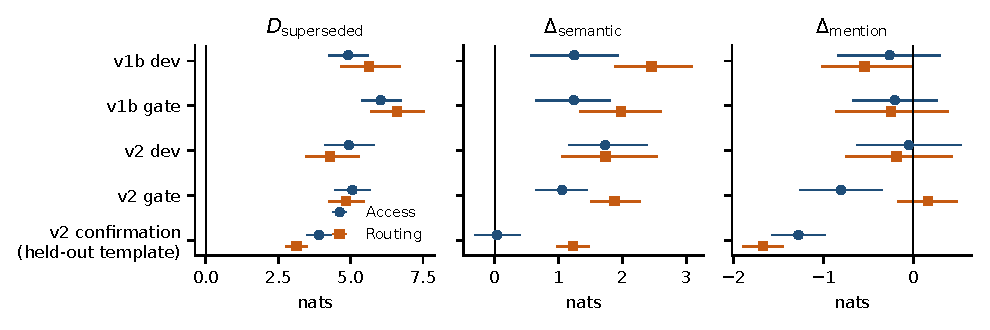
\includegraphics[width=\textwidth]{figures/replication.pdf}
\caption{Primary and mention contrasts across all five splits run under the v1b and v2 protocols (95\%
intervals for development and gate splits, 97.5\% for the confirmation's primary contrasts and 95\% for
its $\Delta_{\mathrm{mention}}$). Development and gate splits used the standard template, and v1b also kept
the \lit{Answer:} line. Only the confirmation is confirmatory.}
\label{fig:replication}
\end{figure*}

\begin{table}[h]
\centering
\small
\setlength{\tabcolsep}{3pt}
\resizebox{\columnwidth}{!}{%
\begin{tabular}{@{}lccc@{}}
\toprule
& Overall & Access & Routing \\
\midrule
Failures & 892/6144 & 454/3072 & 438/3072 \\
Log loss, prevalence & 0.414 & 0.419 & 0.410 \\
Log loss, pre-decision & 0.346 & 0.323 & 0.358 \\
AUROC, pre-decision & 0.780 & 0.834 & 0.729 \\
AUROC, $+R_{\mathrm{easy}}$ & 0.779 & 0.833 & 0.730 \\
Gain from $R_{\mathrm{easy}}$ & $+0.0004$ & $-0.0006$ & $+0.0013$ \\
\bottomrule
\end{tabular}}
\caption{H3: out-of-fold prediction of strict downstream failure on historical-construction items
(history-grouped five-fold cross-validation). 95\% intervals for the gain: overall $[-0.0011, 0.0019]$,
access $[-0.0020, 0.0008]$, routing $[-0.0022, 0.0047]$. The decision's own action confidence, a contemporaneous
reference that is not available before the decision, reaches AUROC 1.000.}
\label{tab:h3}
\end{table}

\begin{table}[h]
\centering
\small
\setlength{\tabcolsep}{3pt}
\begin{tabular}{@{}llcccc@{}}
\toprule
Model & Cell & Direct & No hist. & History & Comp. \\
\midrule
Qwen3-8B & routing seq. & 0.977 & 0.938 & 0.779 & yes \\
 & routing int. & 0.986 & 0.938 & 0.779 & yes \\
 & routing comp. & 0.945 & 0.938 & 0.752 & no \\
 & access seq. & 0.889 & 0.906 & 0.822 & no \\
 & access int. & 0.953 & 0.938 & 0.877 & yes \\
 & access comp. & 0.953 & 0.859 & 0.883 & no \\
\midrule
Qwen3-14B & routing seq. & 0.996 & 0.922 & 0.854 & yes \\
 & routing int. & 1.000 & 1.000 & 0.846 & yes \\
 & routing comp. & 0.997 & 1.000 & 0.814 & yes \\
 & access seq. & 0.991 & 0.781 & 0.729 & no \\
 & access int. & 0.977 & 0.828 & 0.748 & no \\
 & access comp. & 0.946 & 0.828 & 0.697 & no \\
\midrule
Gemma 3 4B & routing seq. & 0.939 & 0.688 & 0.645 & no \\
 & routing int. & 0.964 & 0.609 & 0.488 & no \\
 & routing comp. & 0.916 & 0.625 & 0.533 & no \\
 & access seq. & 0.945 & 0.719 & 0.678 & no \\
 & access int. & 0.936 & 0.609 & 0.676 & no \\
 & access comp. & 0.946 & 0.672 & 0.641 & no \\
\bottomrule
\end{tabular}
\caption{Frozen gate split (384 histories, identical rows for every model): strict direct current-state retrieval, current-only decision accuracy, decision accuracy with history, and whether the cell is competent (direct $\ge 0.95$, no history $\ge 0.90$, invalid $\le 0.05$). This gate decided eligibility to generate confirmation data. Labels computed on the confirmation data (Table~\ref{tab:competence}, Table~\ref{tab:cross-model}) can differ: Qwen3-8B access int. is competent here and not competent on the confirmation data; Qwen3-8B routing comp. is not competent here and competent on the confirmation data.}
\label{tab:models-gate}
\end{table}


\begin{table}[h]
\centering
\small
\setlength{\tabcolsep}{3pt}
\begin{tabular}{@{}llccc@{}}
\toprule
Model & Construction & Kept & Net switch rate & Switched \\
\midrule
Qwen3-8B & superseded & 348/384 & $+0.158$ {\scriptsize $[+0.118, +0.198]$} & 58 / 3 \\
 & other attr. & 357/384 & $+0.048$ {\scriptsize $[+0.014, +0.084]$} & 29 / 12 \\
 & mention & 349/384 & $+0.278$ {\scriptsize $[+0.232, +0.327]$} & 97 / 0 \\
 & unattached & 351/384 & $+0.034$ {\scriptsize $[+0.009, +0.060]$} & 17 / 5 \\
\midrule
Qwen3-14B & superseded & 376/384 & $+0.165$ {\scriptsize $[+0.128, +0.205]$} & 65 / 3 \\
 & other attr. & 367/384 & $+0.136$ {\scriptsize $[+0.101, +0.174]$} & 52 / 2 \\
 & mention & 363/384 & $+0.168$ {\scriptsize $[+0.132, +0.207]$} & 61 / 0 \\
 & unattached & 375/384 & $+0.024$ {\scriptsize $[+0.000, +0.051]$} & 16 / 7 \\
\bottomrule
\end{tabular}
\caption{Routing histories the model demonstrably tracks (criteria of Table~\ref{tab:joint}), per model and construction. Condition (ii), initial-state retrieval, is asked only on the superseded members and is applied at the history level to all four constructions. Net switch rate with 95\% history-bootstrap intervals; switched: histories switched to the wrong / to the correct action.}
\label{tab:joint-by-model}
\end{table}


\begin{figure*}[t]
\centering
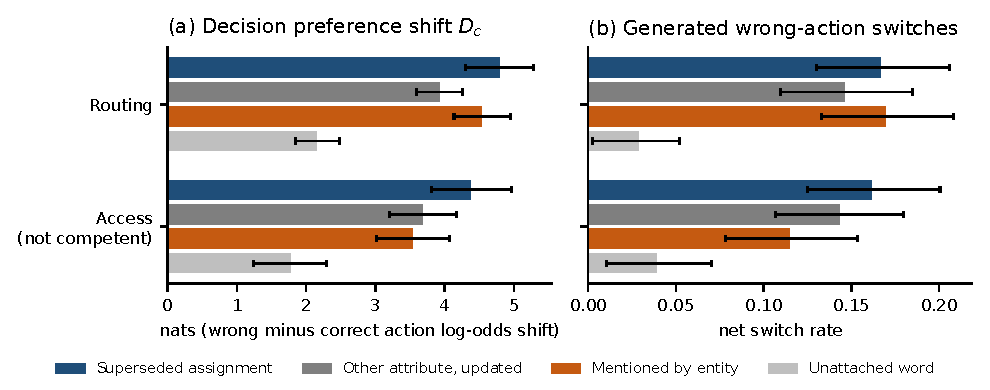
\includegraphics[width=\textwidth]{figures/constructions_qwen3_14b.pdf}
\caption{Qwen3-14B: decision effects by construction (confirmation, 384 histories per task, 95\%
history-bootstrap intervals), as in Figure~\ref{fig:constructions}. Routing cells meet the competence criteria on the confirmation data; access cells do not.}
\label{fig:constructions-14b}
\end{figure*}

\section{Reproducibility}
\label{app:repro}

\paragraph{Models.} Qwen3-8B, Hugging Face revision \lit{b968826d9c46dd6066d109eabc6255188de91218}; Qwen3-14B,
revision \lit{40c069824f4251a91eefaf281ebe4c544efd3e18}; Gemma 3 4B (instruction-tuned), revision
\lit{093f9f388b31de276ce2de164bdc2081324b9767}. All ran in float32 without
quantization, with SDPA attention, on one 80\,GB H100 GPU, using Transformers \citep{wolf2020transformers}
and PyTorch \citep{paszke2019pytorch}. Licenses: Qwen3 (Apache 2.0) and Gemma 3 (Gemma Terms of Use), used for
non-commercial research within their terms.

\paragraph{Artifacts.} Each dataset is regenerated deterministically from its seed and checked against
its manifest. Each score file carries per-record checksums and a completion record binding the scores,
retrieval scores, run manifest, tokenizer audit, code hash and configuration hash. Analyses refuse
incomplete or altered runs. Confirmation: seed 82003, dataset hash
\lit{3e972257\ldots}, code hash \lit{c6648aba\ldots}, configuration hash \lit{78d09215\ldots}, score file
SHA-256 \lit{b159b727\ldots}. The protocol was frozen on 2026-10-08 (UTC), before the gate and
confirmation splits were generated. Every number and figure in this paper is produced from the sealed
analysis reports by one script, which records the hash of each input.

\paragraph{Compute.} Qwen3-8B's confirmation scoring took 6.27 GPU hours (2.67 s per record, including two
retrieval queries, one historical query where applicable, two scored action events and greedy
generation). Qwen3-14B took 1.12 (development), 2.23 (gate) and 4.48 GPU hours (confirmation), 1.91 s per
confirmation record. Both runs used the same GPU type, software versions (PyTorch 2.14.0, Transformers
5.17.0), scorer and prompts (mean 199 prompt tokens). The times are wall-clock as logged. We did not record
GPU sharing or clock state, so we cannot attribute the faster per-record time of the larger model. The
whole program, including failed runs, development and gate splits and the ineligible model, used about
32 GPU hours.

\paragraph{Code.} The anonymized archive submitted as supplementary software contains the generators,
scoring and analysis code, tests, configuration files, the dated protocol records, the sealed analysis
reports with their run records, the confirmation datasets and per-record scores of both confirmed models,
and the scripts that derive every number, table and figure in this paper; run from the archive, they
reproduce the paper's derived values exactly.


\end{document}
